\documentclass[12pt,letterpaper]{article}
\usepackage[utf8]{inputenc}
\usepackage[spanish,mexico]{babel}
\usepackage{amsmath}
\usepackage{amsfonts}
\usepackage{amssymb}
\usepackage{amsmath}
\usepackage[lmargin=3cm,rmargin=3cm,tmargin=3cm,bmargin=3cm]{geometry}

\usepackage{hyperref}
\usepackage{graphicx}
\usepackage{float}


\begin{document}

\title{Actividad 10: Animación del Péndulo y espacio Fase}
\author{Luisa Fernanda Orci Fernandez.}
\date{20 de Abril del 2016}

\maketitle

\section*{Actividad}

Para esta actividad se nos pidió realizar dos animaciones similares a las que salen en el artículo de Wikipedia sobre el Péndulo\cite{1}. Estas dos son un péndulo simple y su espacio fase. \\
Para poder llevar a cabo esta actividad, nos apoyamos en la biblioteca de $Matplotlib$ de $Python$; nos basamos en algunos de sus ejemplos y los adaptamos para poder crear nuestras propias animaciones. \\

\subsection*{Péndulo Simple}
Para la parte de la animación del movimiento en el espacio del péndulo simple, utilizamos el cógido ejemplo proporcionado por $Matplotlib$: 

\begin{verbatim}
# Double pendulum formula translated from the C code at
# http://www.physics.usyd.edu.au/~wheat/dpend_html/solve_dpend.c

from numpy import sin, cos
import numpy as np
import matplotlib.pyplot as plt
import scipy.integrate as integrate
import matplotlib.animation as animation

G = 9.8  # acceleration due to gravity, in m/s^2
L1 = 1.0  # length of pendulum 1 in m
L2 = 1.0  # length of pendulum 2 in m
M1 = 1.0  # mass of pendulum 1 in kg
M2 = 1.0  # mass of pendulum 2 in kg


def derivs(state, t):

    dydx = np.zeros_like(state)
    dydx[0] = state[1]

    del_ = state[2] - state[0]
    den1 = (M1 + M2)*L1 - M2*L1*cos(del_)*cos(del_)
    dydx[1] = (M2*L1*state[1]*state[1]*sin(del_)*cos(del_) +
               M2*G*sin(state[2])*cos(del_) +
               M2*L2*state[3]*state[3]*sin(del_) -
               (M1 + M2)*G*sin(state[0]))/den1

    dydx[2] = state[3]

    den2 = (L2/L1)*den1
    dydx[3] = (-M2*L2*state[3]*state[3]*sin(del_)*cos(del_) +
               (M1 + M2)*G*sin(state[0])*cos(del_) -
               (M1 + M2)*L1*state[1]*state[1]*sin(del_) -
               (M1 + M2)*G*sin(state[2]))/den2

    return dydx

# create a time array from 0..100 sampled at 0.05 second steps
dt = 0.05
t = np.arange(0.0, 20, dt)

# th1 and th2 are the initial angles (degrees)
# w10 and w20 are the initial angular velocities (degrees per second)
th1 = 120.0
w1 = 0.0
th2 = -10.0
w2 = 0.0

# initial state
state = np.radians([th1, w1, th2, w2])

# integrate your ODE using scipy.integrate.
y = integrate.odeint(derivs, state, t)

x1 = L1*sin(y[:, 0])
y1 = -L1*cos(y[:, 0])

x2 = L2*sin(y[:, 2]) + x1
y2 = -L2*cos(y[:, 2]) + y1

fig = plt.figure()
ax = fig.add_subplot(111, autoscale_on=False, xlim=(-2, 2), ylim=(-2, 2))
ax.grid()

line, = ax.plot([], [], 'o-', lw=2)
time_template = 'time = %.1fs'
time_text = ax.text(0.05, 0.9, '', transform=ax.transAxes)


def init():
    line.set_data([], [])
    time_text.set_text('')
    return line, time_text


def animate(i):
    thisx = [0, x1[i], x2[i]]
    thisy = [0, y1[i], y2[i]]

    line.set_data(thisx, thisy)
    time_text.set_text(time_template % (i*dt))
    return line, time_text

ani = animation.FuncAnimation(fig, animate, np.arange(1, len(y)),
                              interval=25, blit=True, init_func=init)

#ani.save('double_pendulum.mp4', fps=15)
plt.show()
\end{verbatim}

Como este código fue diseñado para hacer una animación de un péndulo doble, como se dijo anteriormente, lo adaptamos de la siguiente forma para que pudiera darnos la animación de un péndulo simple, dándole valores de $0$ a la longitud y a la masa del segundo péndulo, también fue necesario eliminar del código las ecuaciones para el segundo péndulo. \\

\begin{verbatim}
from numpy import sin, cos
import numpy as np
import matplotlib.pyplot as plt
import scipy.integrate as integrate
import matplotlib.animation as animation
import math

class DoublePendulum:
    """Double Pendulum Class

    init_state is [theta1, omega1, theta2, omega2] in degrees,
    where theta1, omega1 is the angular position and velocity of the first
    pendulum arm, and theta2, omega2 is that of the second pendulum arm
    """
    def __init__(self,
                 init_state = [120, 0, -20, 0],
                 L1=1.0,  # length of pendulum 1 in m
                 L2=1.0,  # length of pendulum 2 in m
                 M1=1.0,  # mass of pendulum 1 in kg
                 M2=1.0,  # mass of pendulum 2 in kg
                 G=9.8,  # acceleration due to gravity, in m/s^2
                 origin=(0, 0)): 
        self.init_state = np.asarray(init_state, dtype='float')
        self.params = (L1, L2, M1, M2, G)
        self.origin = origin
        self.time_elapsed = 0

        self.state = self.init_state * np.pi / 180.
    
    def position(self):
        """compute the current x,y positions of the pendulum arms"""
        (L1, L2, M1, M2, G) = self.params

        x = np.cumsum([self.origin[0],
                       L1 * sin(self.state[0]),
                       L2 * sin(self.state[2])])
        y = np.cumsum([self.origin[1],
                       -L1 * cos(self.state[0]),
                       -L2 * cos(self.state[2])])
        return (x, y)

    def energy(self):
        """compute the energy of the current state"""
        (L1, L2, M1, M2, G) = self.params

        x = np.cumsum([L1 * sin(self.state[0]),
                       L2 * sin(self.state[2])])
        y = np.cumsum([-L1 * cos(self.state[0]),
                       -L2 * cos(self.state[2])])
        vx = np.cumsum([L1 * self.state[1] * cos(self.state[0]),
                        L2 * self.state[3] * cos(self.state[2])])
        vy = np.cumsum([L1 * self.state[1] * sin(self.state[0]),
                        L2 * self.state[3] * sin(self.state[2])])

        U = G * (M1 * y[0] + M2 * y[1])
        K = 0.5 * (M1 * np.dot(vx, vx) + M2 * np.dot(vy, vy))

        return U + K

    def dstate_dt(self, state, t):
        """compute the derivative of the given state"""
        (M1, M2, L1, L2, G) = self.params

        dydx = np.zeros_like(state)
        dydx[0] = state[1]
        dydx[2] = state[3]

        cos_delta = cos(state[2] - state[0])
        sin_delta = sin(state[2] - state[0])

        den1 = (M1 + M2) * L1 - M2 * L1 * cos_delta * cos_delta
        dydx[1] = (M2 * L1 * state[1] * state[1] * sin_delta * cos_delta
                   + M2 * G * sin(state[2]) * cos_delta
                   + M2 * L2 * state[3] * state[3] * sin_delta
                   - (M1 + M2) * G * sin(state[0])) / den1

        den2 = (L2 / L1) * den1
        dydx[3] = (-M2 * L2 * state[3] * state[3] * sin_delta * cos_delta
                   + (M1 + M2) * G * sin(state[0]) * cos_delta
                   - (M1 + M2) * L1 * state[1] * state[1] * sin_delta
                   - (M1 + M2) * G * sin(state[2])) / den2
        
        return dydx

    def step(self, dt):
        """execute one time step of length dt and update state"""
        self.state = integrate.odeint(self.dstate_dt, self.state, [0, dt])[1]
        self.time_elapsed += dt

#------------------------------------------------------------
# set up initial state and global variables
pendulum = DoublePendulum([180, 0.0, -20., 0.0], L2=0)
dt = 1./30 # 30 fps

#------------------------------------------------------------
# set up figure and animation
fig = plt.figure()


ax1 = fig.add_subplot(2, 1, 1)
ax = fig.add_subplot(212, aspect='equal', autoscale_on=False,
                     #)
                     xlim=(-2, 2), ylim=(-2, 4))

ax.grid()

line, = ax.plot([], [], 'o-', lw=2)
time_text = ax.text(0.02, 0.95, '', transform=ax.transAxes)
energy_text = ax.text(0.02, 0.90, '', transform=ax.transAxes)
position_text = ax.text(0.02, 0.85, '', transform=ax.transAxes)

def init():
    """initialize animation"""
    line.set_data([], [])
    time_text.set_text('')
    energy_text.set_text('')
    position_text.set_text('')
    return line, time_text, energy_text, position_text

def animate(i):
    """perform animation step"""
    global pendulum, dt
    pendulum.step(dt)
    

    line.set_data(*pendulum.position())
    var = line.get_data()
    #print var
    #print var[0][1], var[1][1]
    time_text.set_text('time = %.1f' % pendulum.time_elapsed)
    energy_text.set_text('energy = %.3f J' % pendulum.energy())
    posx = var[0][1]
    posy = var[1][1]
    angle = math.atan(posy/posx)
    angle = angle / (np.pi / 180)
    position_text.set_text('Ang= %.3f Pos = %.3f, %.3f' % (angle, posx, posy))
    
    return line, time_text, energy_text, position_text

# choose the interval based on dt and the time to animate one step
from time import time
t0 = time()
animate(0)
t1 = time()
interval = 1000 * dt - (t1 - t0)
#ani = animation.FuncAnimation(fig, animate, frames=300,
#                              interval=interval, blit=True, init_func=init)
ani = animation.FuncAnimation(fig, animate, frames=300,
                              interval=interval*5, blit=True, init_func=init)

# save the animation as an mp4.  This requires ffmpeg or mencoder to be
# installed.  The extra_args ensure that the x264 codec is used, so that
# the video can be embedded in html5.  You may need to adjust this for
# your system: for more information, see
# http://matplotlib.sourceforge.net/api/animation_api.html
#ani.save('double_pendulum.mp4', fps=30, extra_args=['-vcodec', 'libx264'])

plt.show()
\end{verbatim}

\subsection*{Espacio Fase}
Para el espacio fase modificamos se nos proporcionó un código y tuvimos que modificarlo y quedó de la siguiente manera:

\begin{verbatim}
import numpy as np
from matplotlib import pyplot as plt
from matplotlib import animation as an
from matplotlib.lines import Line2D
from scipy.integrate import odeint

#Definiendo las constantes de la Ec. Diferencial
g = 9.81
l = 1.0
b = 0.0 #Pendulo simple por lo tanto sin friccion
c = g/l

#Codiciones Iniciales
X_f1 =np.array([(180.0/180.0)*np.pi,(-250./180.0)*np.pi])
t = np.linspace(-0.0*np.pi,5.0*np.pi,500) #Para generar la solucion

#Definicion de la ecuacion diderencial del pendulo
def p (y, t, b, c):
    theta, omega = y
    dy_dt = [omega,-b*omega -c*np.sin(theta)]
    return dy_dt

#=====================================
# Trayectoria
y0 = X_f1                               # Punto de Inicio   
X = odeint(p, y0, t, args=(b,c))         

#=====================================
#Graficar

class SubplotAnimation(an.TimedAnimation):
    def __init__(self):
        fig = plt.figure()
        ax1 = fig.add_subplot(1, 1, 1)
       
        self.t = np.linspace(0, 80, 400)
        self.x = X[:,0]
        self.y = X[:,1]

        self.line1 = Line2D([], [], color='black')
        self.line1a = Line2D([], [], color='red', linewidth=2)
        self.line1e = Line2D(
            [], [], color='red', marker='o', markeredgecolor='r')
        ax1.add_line(self.line1)
        ax1.add_line(self.line1a)
        ax1.add_line(self.line1e)
        ax1.set_xlim(-10, 10)
        ax1.set_ylim(-10, 10)
        ax1.set_aspect('equal', 'datalim')

        an.TimedAnimation.__init__(self, fig, interval=50, blit=True)

    def _draw_frame(self, framedata):
        i = framedata
        head = i - 1
        #head_len = 10
        head_slice = (self.t > self.t[i] - 1.0) & (self.t < self.t[i])

        self.line1.set_data(self.x[:i], self.y[:i])
        self.line1a.set_data(self.x[head_slice], self.y[head_slice])
        self.line1e.set_data(self.x[head], self.y[head])

    def new_frame_seq(self):
        return iter(range(self.t.size))

    def _init_draw(self):
        lines = [self.line1, self.line1a, self.line1e]
        for l in lines:
            l.set_data([], [])

ani = SubplotAnimation()
#ani.save('test_sub.mp4')
plt.show()
\end{verbatim}

\subsection*{Casos Especificos}

\subsubsection*{$\theta = 0$}
Péndulo:
\begin{center}
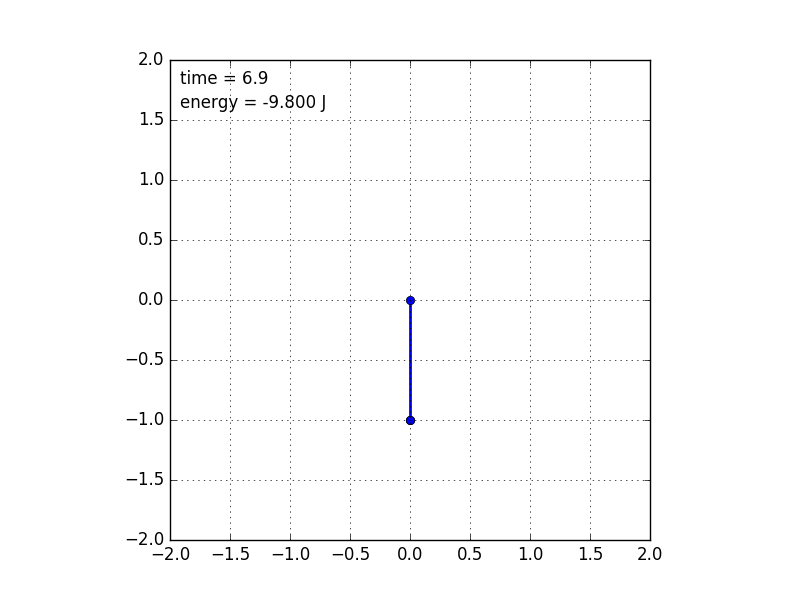
\includegraphics[scale=0.3]{0.png}
\end{center}
Espacio fase:
\begin{center}
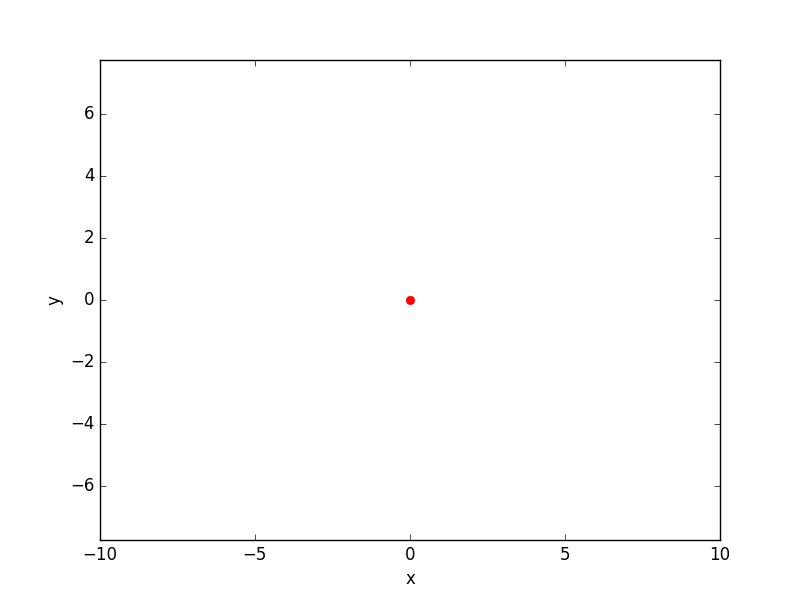
\includegraphics[scale=0.3]{01.png}
\end{center}

\subsubsection*{$\theta = 45$}
Péndulo:
\begin{center}
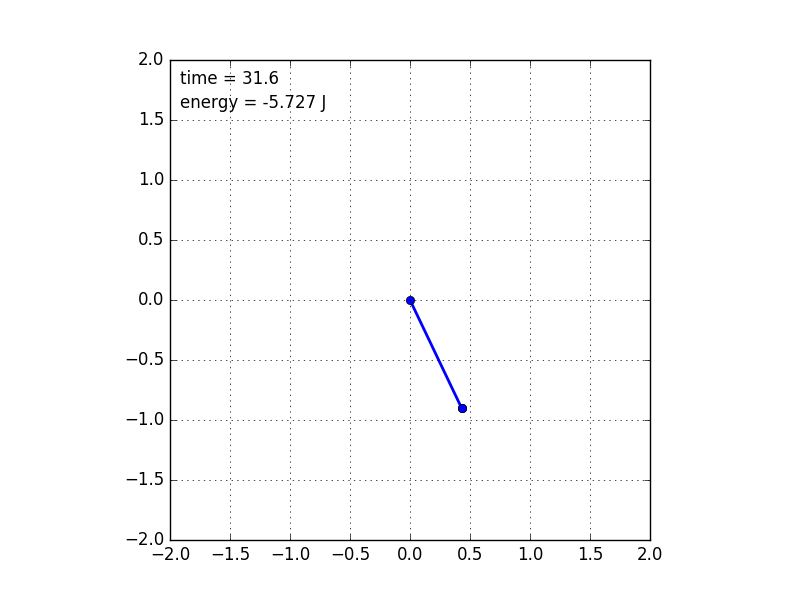
\includegraphics[scale=0.3]{451.png}
\end{center}
Espacio fase:
\begin{center}
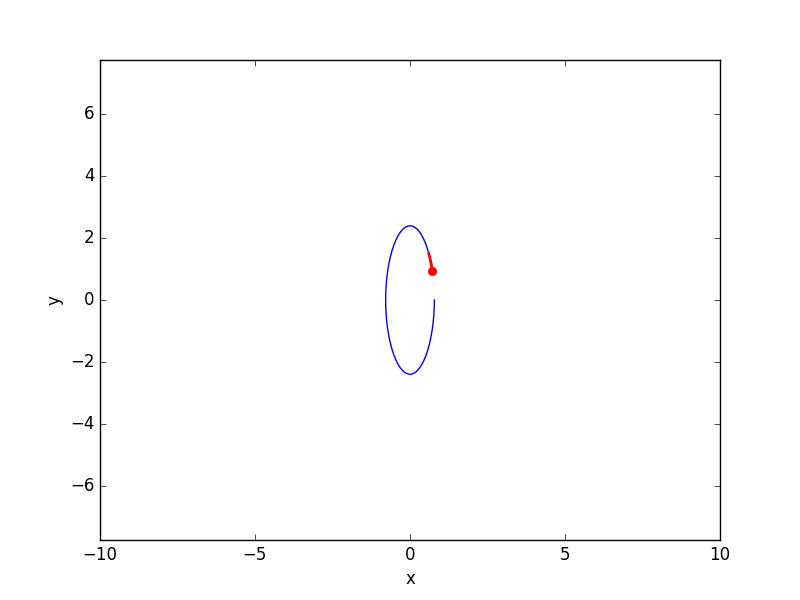
\includegraphics[scale=0.3]{45.png}
\end{center}

\subsubsection*{$\theta = 90$}
Péndulo:
\begin{center}
%\includegraphics[scale=0.3]{•}
\end{center}
Espacio fase:
\begin{center}
%\includegraphics[scale=0.3]{•}
\end{center}

\subsubsection*{$\theta = 135$}
Péndulo:
\begin{center}
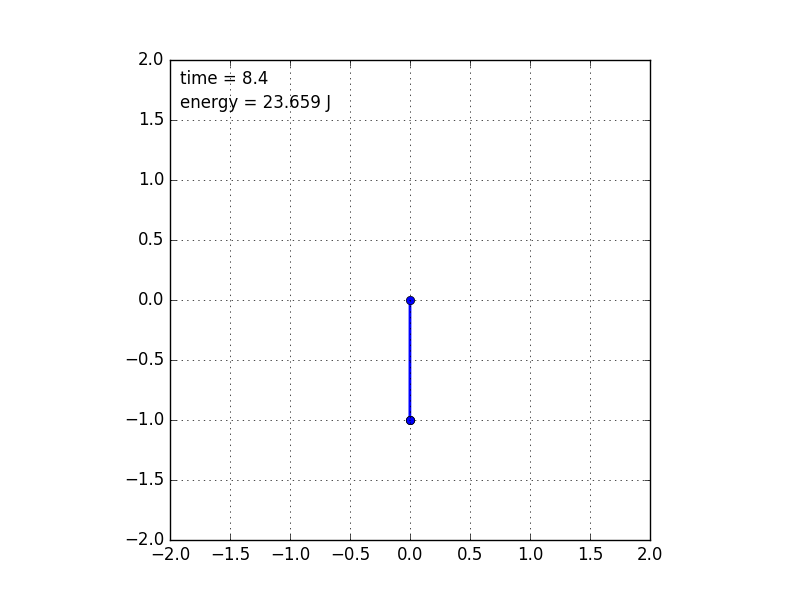
\includegraphics[scale=0.3]{135.png}
\end{center}
Espacio fase:
\begin{center}
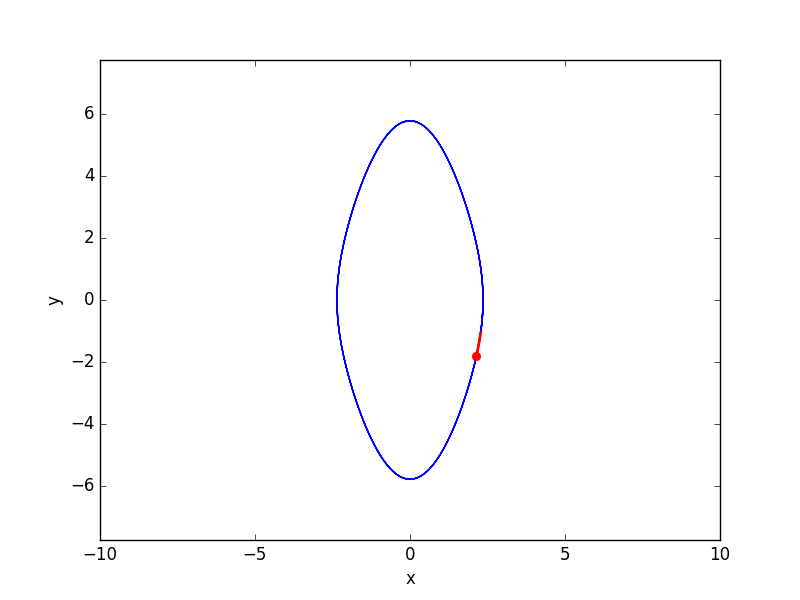
\includegraphics[scale=0.3]{1351.png}
\end{center}

\subsubsection*{$\theta = 170$}
Péndulo:
\begin{center}
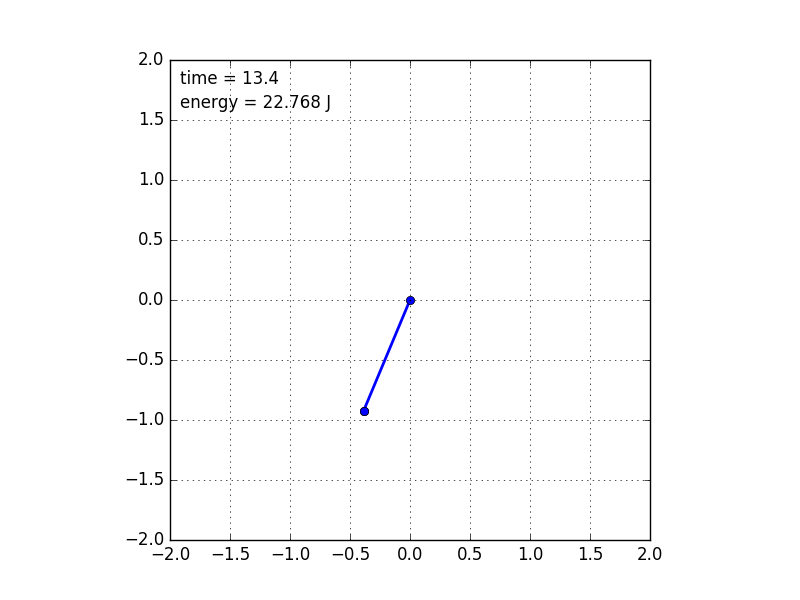
\includegraphics[scale=0.3]{170.png}
\end{center}
Espacio fase:
\begin{center}
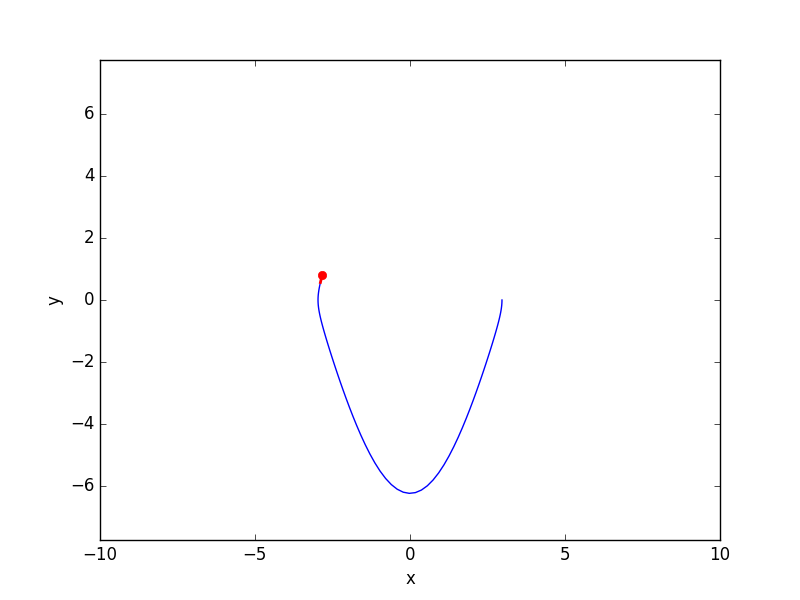
\includegraphics[scale=0.3]{1701_.png}
\end{center}

\subsubsection*{$\theta = 180$}
Péndulo:
\begin{center}
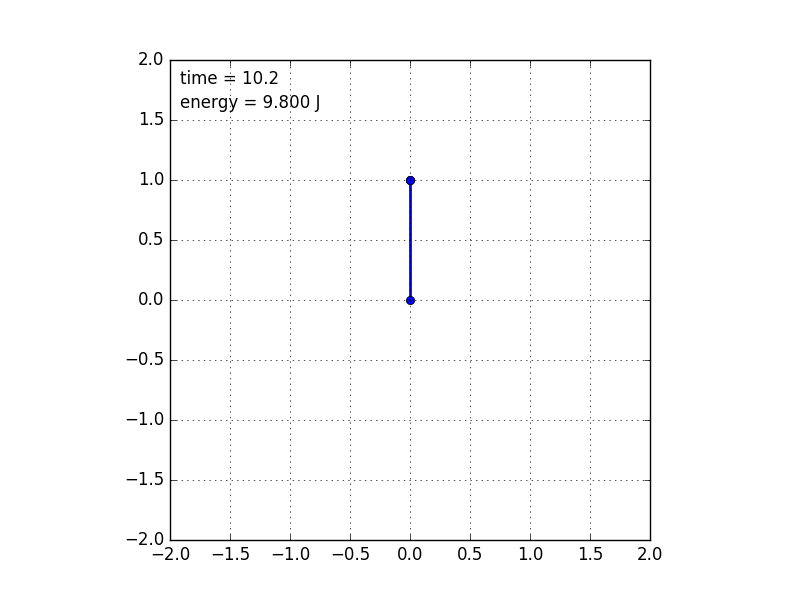
\includegraphics[scale=0.3]{180.png}
\end{center}
Espacio fase:
\begin{center}
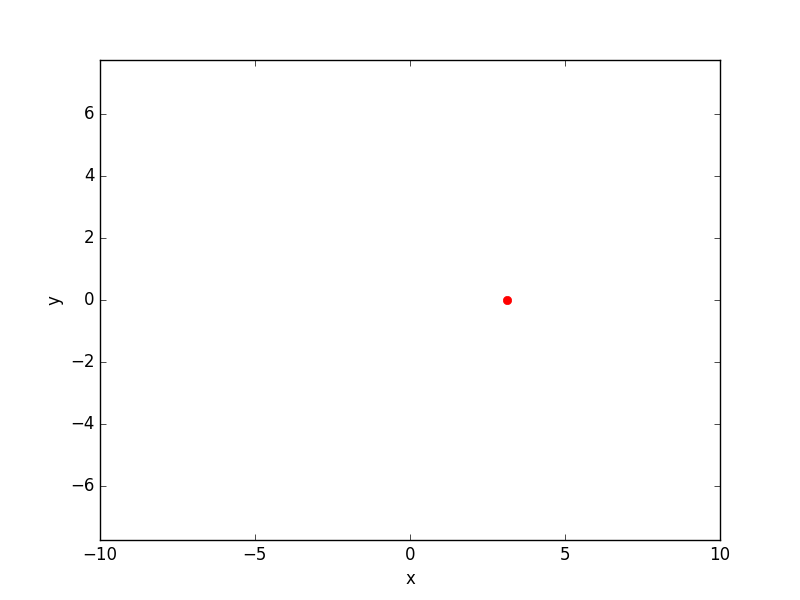
\includegraphics[scale=0.3]{1801.png}
\end{center}

\subsubsection*{Ejemplo extra 1}
Péndulo:
\begin{center}
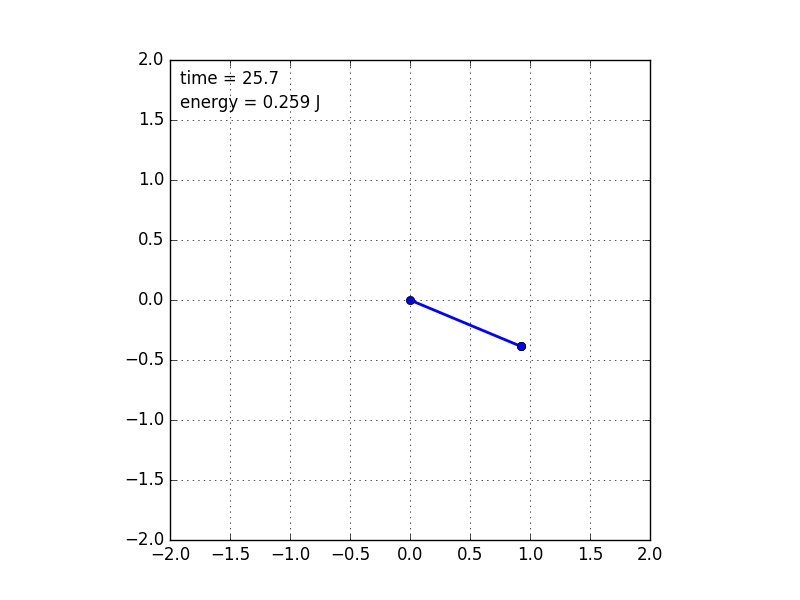
\includegraphics[scale=0.3]{E.png}
\end{center}
Espacio fase:
\begin{center}
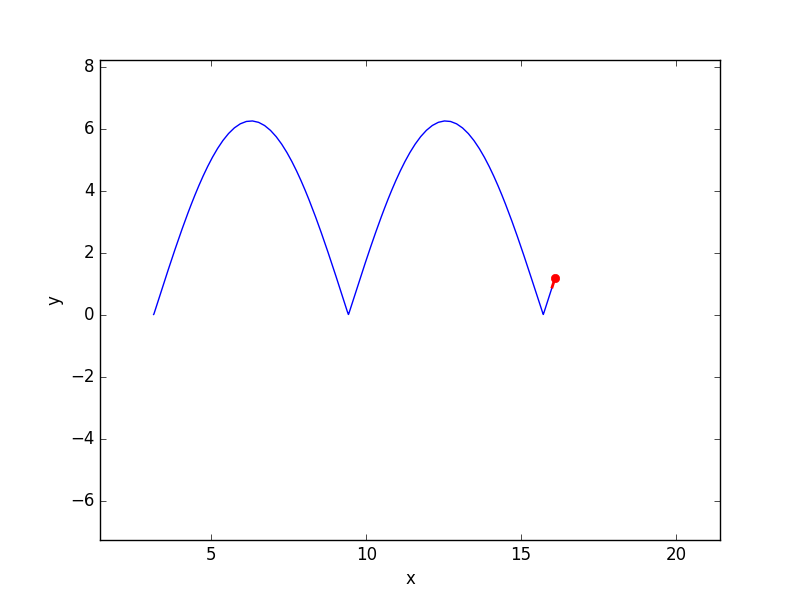
\includegraphics[scale=0.3]{E1.png}
\end{center}

\subsubsection*{Ejemplo extra 2}
Péndulo:
\begin{center}
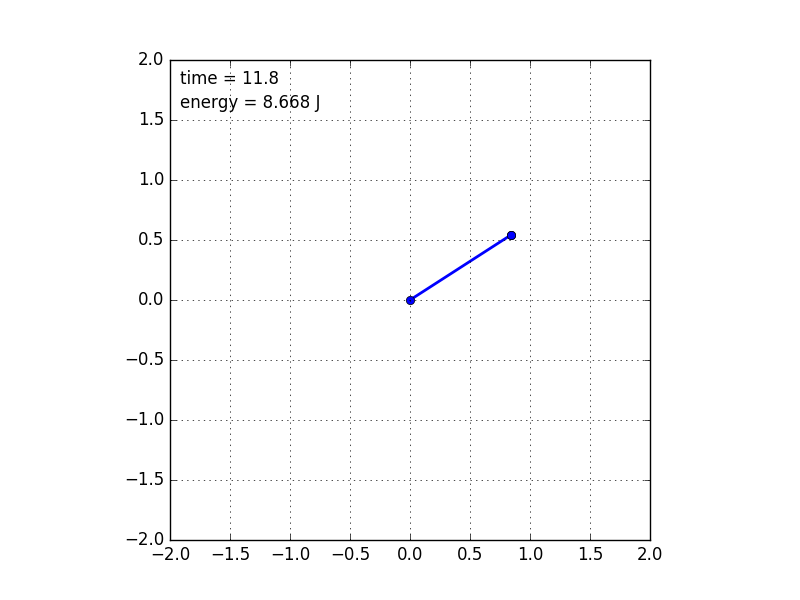
\includegraphics[scale=0.3]{e.png}
\end{center}
Espacio fase:
\begin{center}
\includegraphics[scale=0.3]{e1.png}
\end{center}

\section{Conclusiones}

Esta actividad representó un gran reto para mi, ya que se me dificultó mucho al momento de moficiar el código y realizar las animaciones, pero una vez que encontré un programa para grabar la pantalla, lo demas se facilitó.\\
Algo muy positivo de esta actividad es que en un futuro será de gran apoyo para realizar animaciones de otros problemas físicos.


\begin{thebibliography}{widestlabel}

\bibitem{1} Wikipedia, la enciclopedia libre \emph{Pendulum}, (2016, 08 de Marzo). Desde: \url{https://en.wikipedia.org/wiki/Pendulum_\%28mathematics\%29#Arbitrary-amplitude_period}

\bibitem{2} Matplotlib \emph{Animation example code: double pendulum}, (2016, 20 de Abril). Desde: \url{http://matplotlib.org/examples/animation/double_pendulum_animated.html}

\bibitem{3} Matplotlib \emph{Animation example code: double pendulum}, (2016, 20 de Abril). Desde: \url{http://matplotlib.org/examples/animation/double_pendulum_animated.html}

\end{thebibliography}

\end{document}